
\chapter{系统实现和实验结果}
\label{chap:experiment}

\section{系统具体实现}
\label{sec:implementation}
我们采用Scala语言来搭建我们的系统。Scala是一种运行在JVM上的静态语言,支持函数式、
面向对象等多种编程范式,可以和Java代码无缝地进行交互。目前Scala还处于不断发展中,
新版本不向后兼容,我们的系统在Scala 2.10上可以编译通过。在工程管理上,我们使
用sbt管理Scala代码的编译和依赖关系。

在系统的实现中我们还使用了许多第三方库,除了在第~\ref{chap:cluster}章中介绍
的Actor库Akka,还有:
\begin{itemize}
\item 日志系统:基于twitter公司开源的util包,地址在
  \url{https://github.com/twitter/util}。
\item 网页字符集检测:ICU4J,地址在\url{http://site.icu-project.org},这是一
  套UNICODE相关的工具集,提供了较好的字符集编码检测功能,我们用于检测中文网页的字
  符集。
\item HTML解析器:jsoup,地址在\url{http://jsoup.org},是一个用Java语言实现
  的HTML解析器,用于DOM Tree的构建和节点内容的抽取。
\end{itemize}
\section{实验演示系统}
\label{sec:demo}
为了直观地显示网页模板的匹配效果,我们基于Play! Framework的Web开发框架实现了一
个Web Service,用于实验的演示。该Web Service的工作原理
如\reffig{experiment:fig:demo}所示。
\begin{figure}
  \centering
  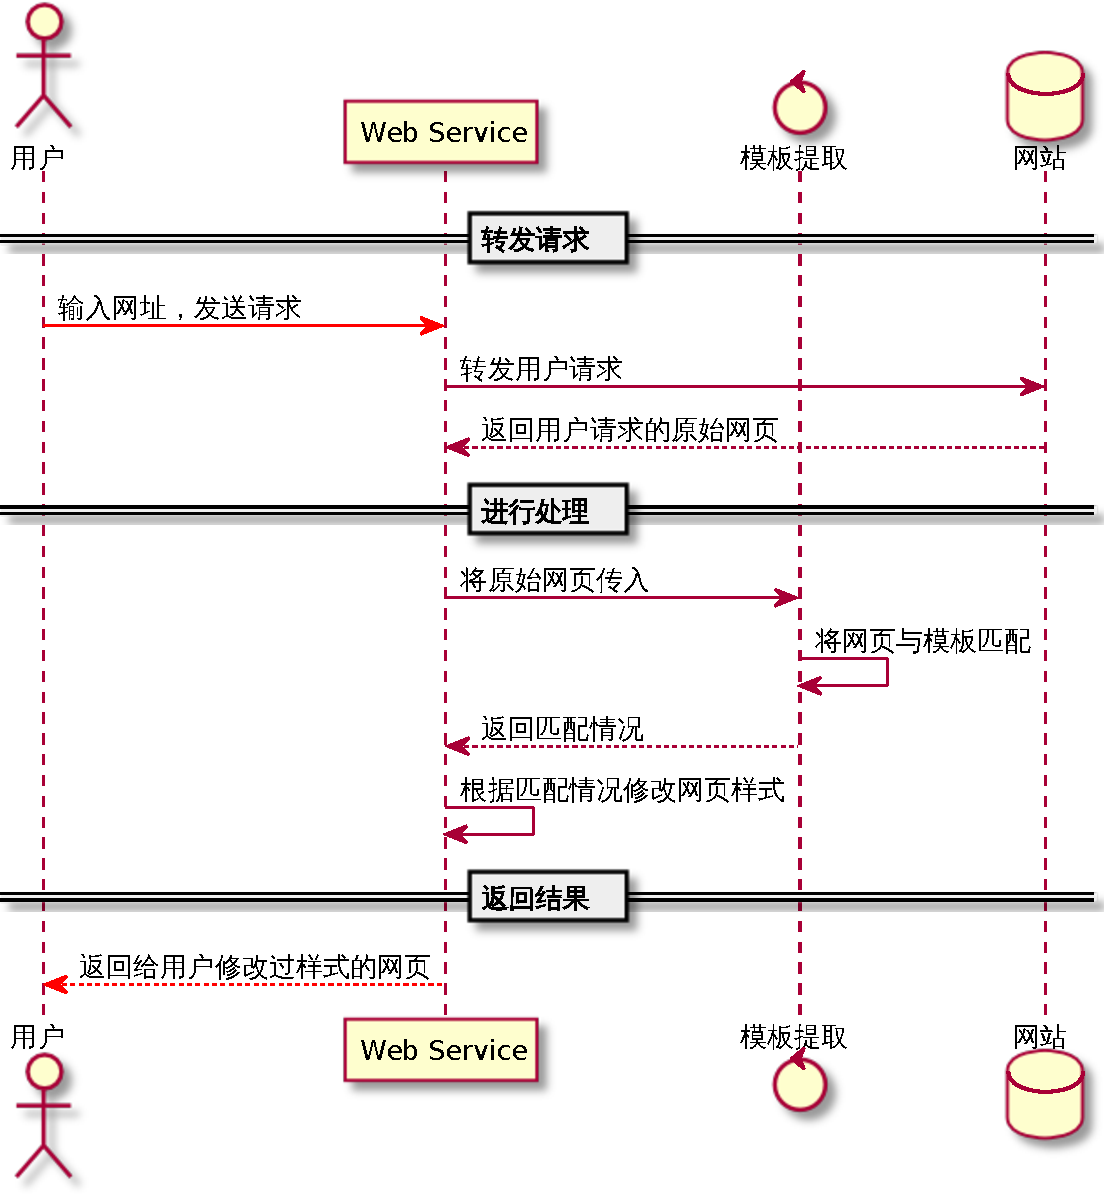
\includegraphics[width=0.75\textwidth]{experiment06/demo}
  \caption{Web Service工作原理}
  \label{experiment:fig:demo}
\end{figure}

用户只需要输入一个需要和系统的模板进行匹配的网页的URL,系统将返回一个修改过样式的
新的网页,使得原网页和模板的匹配情况可以从浏览器中直观地看到。
% TODO: 实验演示的效果如\reffig{experiment:fig:demoresult}所示
% \begin{figure}
%   \centering
%   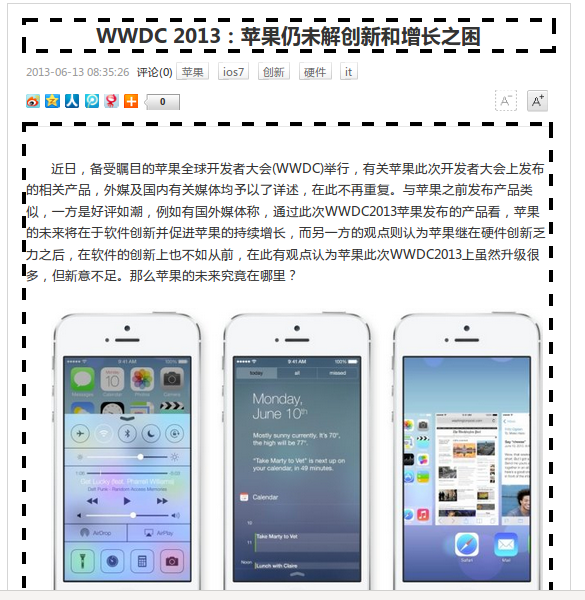
\includegraphics[width=0.5\textwidth]{experiment06/demoresult}
%   \caption{实验演示系统效果}
%   \label{experiment:fig:demoresult}
% \end{figure}
\section{实验环境和数据}
\label{sec:dataenv}
我们实验所用的机器的配置情况是:16个逻辑核的CPU,24G内存,操作系统为64位的CentOS。
后续的实验均在这个机器上进行。

我们有三个实验数据集,分别为博客(blog),新闻(news)和其他(others)。实验数据
集的概况如\reftbl{experiment:tab:overview}所示。%TODO
\begin{table}[h]
  \centering
% BEGIN RECEIVE ORGTBL 实验数据概况
\begin{tabular}{llll}
\toprule
 & blog & news & other \\
\hline
文件个数 & 59998 & 81561 & 183635 \\
总大小 & 5.4G & 7.9G & 18G \\
来源 & blog.sina.com.cn &  news.xxx.com &  \\
\bottomrule
\end{tabular}
% END RECEIVE ORGTBL 实验数据概况
  \caption{实验数据概况}
  \label{experiment:tab:overview}
\end{table}
\begin{comment}
#+ORGTBL: SEND 实验数据概况 orgtbl-to-latex :splice nil :skip 0
|          | blog             | news  | other  |
|----------+------------------+-------+--------|
| 文件个数 | 59998            | 81561 | 183635 |
| 总大小   | 5.4G             | 7.9G  | 18G    |
| 来源     | blog.sina.com.cn |       |        |
\end{comment}

接下来的几个小节我们将大体按照模块的顺序,依次介绍实验的详细情况。
\label{sec:results}
\section{预处理模块实验与分析}
\label{sec:experiement:pre}
在预处理模块中,我们首先将过滤掉无用的网页,包括目录页和错误页,采用的是
第~\ref{sec:filterintro-useless}节中介绍的基于规则的方
法。\reftbl{experiment:tab:filter}给出了实验中使用的过滤规则和对应的结果。%TODO
\begin{table}[hb]
  \centering
% BEGIN RECEIVE ORGTBL 过滤无用网页
\begin{tabular}{lrrr}
  \toprule
 & blog & news & others \\
\hline
目录页URL规则 & .*(?<!\textbackslash\textbackslash.html?)\$ & .*(?<!\textbackslash\textbackslash.shtml)\$ &  \\
错误页最大长度 & 6000 & 6000 &  \\
文件个数 & 59998 & 81561 & 183635 \\
过滤后详细页个数 &  &  &  \\
\bottomrule
\end{tabular}
% END RECEIVE ORGTBL 过滤无用网页
  \caption{过滤无用网页实验结果}
  \label{experiment:tab:filter}
\end{table}
\begin{comment}
#+ORGTBL: SEND 过滤无用网页 orgtbl-to-latex :splice nil :skip 0
|                  |                                       blog |                                       news | others |
|------------------+--------------------------------------------+--------------------------------------------+--------|
| 目录页URL规则    | .*(?<!\textbackslash\textbackslash.html?)$ | .*(?<!\textbackslash\textbackslash.shtml)$ |        |
| 错误页最大长度   |                                       6000 |                                       6000 |        |
| 原来总文件个数   |                                      59998 |                                      81561 | 183635 |
| 过滤后详细页个数 |                                            |                                            |        |
\end{comment}

过滤掉了不需要的网页以后,我们得到了详细页的集合。在进行下一步的实验之前,我们将
这些详细页集合分成训练集和测试集,各个数据集的具体分割情况如
\reftbl{experiment:tab:split}所示。%TODO
\begin{table}[hb]
\centering
% BEGIN RECEIVE ORGTBL 数据分割
\begin{tabular}{llll}
  \toprule
 & 训练集 & 测试集 & 详细页总数 \\
\hline
blog &  &  &  \\
news &  &  &  \\
others &  &  &  \\
\bottomrule
\end{tabular}
% END RECEIVE ORGTBL 数据分割
\caption{训练集和测试集分布}
\label{experiment:tab:split}
\end{table}
\begin{comment}
#+ORGTBL: SEND 数据分割 orgtbl-to-latex :splice nil :skip 0
|        | 训练集 | 测试集 | 详细页总数 |
|--------+--------+--------+------------|
| blog   |        |        |            |
| news   |        |        |            |
| others |        |        |            |
\end{comment}

接下来将所有的无用标签,\reftbl{experiment:tab:uselesstags}给出了我们实验中去掉的
所有无用标签以及对应的正则表达式模式。
\begin{table}[hb]
  \centering
% BEGIN RECEIVE ORGTBL 无用标签
\begin{tabular}{ll}
  \toprule
正则表达式模式 & 对应的标签名 \\
\hline
(?is)<tag.*?>.*?</tag> & style,script \\
(?is)<[/]?tag.*?> & link,input,br,img,meta,wbr \\
(?is)<[/]?tag.*?> & strong,em,font,b,p,li,ul,ol,td,tr,th,tbody,table \\
\bottomrule
\end{tabular}
% END RECEIVE ORGTBL 无用标签
  \caption{去掉的无用标签}
  \label{experiment:tab:uselesstags}
\end{table}
\begin{comment}
#+ORGTBL: SEND 无用标签 orgtbl-to-latex :splice nil :skip 0
| 正则表达式模式         | 对应的标签名                                     |
|------------------------+--------------------------------------------------|
| (?is)<tag.*?>.*?</tag> | style,script                                     |
| (?is)<[/]?tag.*?>      | link,input,br,img,meta,wbr                       |
| (?is)<[/]?tag.*?>      | strong,em,font,b,p,li,ul,ol,td,tr,th,tbody,table |
\end{comment}

下面我们对后缀树检测重复记录的算法进行一些实验。我们统计每个数据集中检测出的重复
记录的按照长度的分布情况,
如\reffig{experiment:fig:recordlength}所示。% TODO
\begin{figure}[hb]
  \centering
  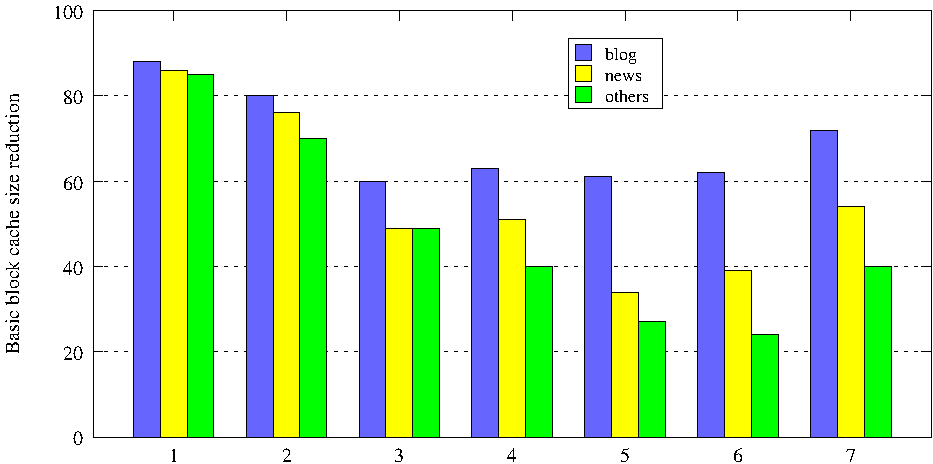
\includegraphics[width=0.8\textwidth]{experiment06/recordlength}
  \caption{检测出的重复记录长度的分布情况}
  \label{experiment:fig:recordlength}
\end{figure}

我们可以看到,大部分的重复记录集中在。% Lorem ipsum dolor sit amet, consectetur adipisicing elit, sed do eiusmod tempor incididunt ut labore et dolore magna aliqua. Ut enimad minim veniam, quis nostrud exercitation ullamco laboris nisi ut aliquip ex ea commodo consequat. Duis aute irure dolor in reprehenderit in voluptate velit esse cillum dolore eu fugiat nulla pariatur. Excepteur sint occaecat cupidatat non proident, sunt in culpa qui officia deserunt mollit anim id est laborum.

\section{聚类和模板生成模块实验和分析}
由于网页的数量非常多,计算网页的结构相似度将是我们整个系统最耗时的部分,因此,我
们先将训练集中所有的文档结构相似度离线算好,方便后续的实
验。\reftbl{experiment:tab:calcsim}给出了在各个数据集上计算所有的文档结构相似度的时间统计结果。 % TODO
\begin{table}[h]
  \centering
% BEGIN RECEIVE ORGTBL 计算时间
\begin{tabular}{llll}
  \toprule
 & blog & news & others \\
\hline
训练集大小 &  &  &  \\
所花时间 &  &  &  \\
\bottomrule
\end{tabular}
% END RECEIVE ORGTBL 计算时间
\caption{每个数据集计算全部文档结构相似度的时间}
\label{experiment:tab:calcsim}
\end{table}
\begin{comment}
#+ORGTBL: SEND 计算时间 orgtbl-to-latex :splice nil :skip 0
|            | blog | news | others |
|------------+------+------+--------|
| 训练集大小 |      |      |        |
| 所花时间   |      |      |        |
\end{comment}

可以看到,由于采用了Actor模型进行并行计算%TODO:分析

在聚类模块中,最重要的实验参数是聚类时设置的相似度阈值。我们调整该阈值,观察聚类
的个数的变化;同时为了进一步看出调整聚类时阈值对后面模板生成模块的影响,我们将生
成的模板的一些统计信息也放入表格中。我们选择在news数据集上进行实验,具体的实验结
果见\reffig{experiment:fig:threshold}。%TODO

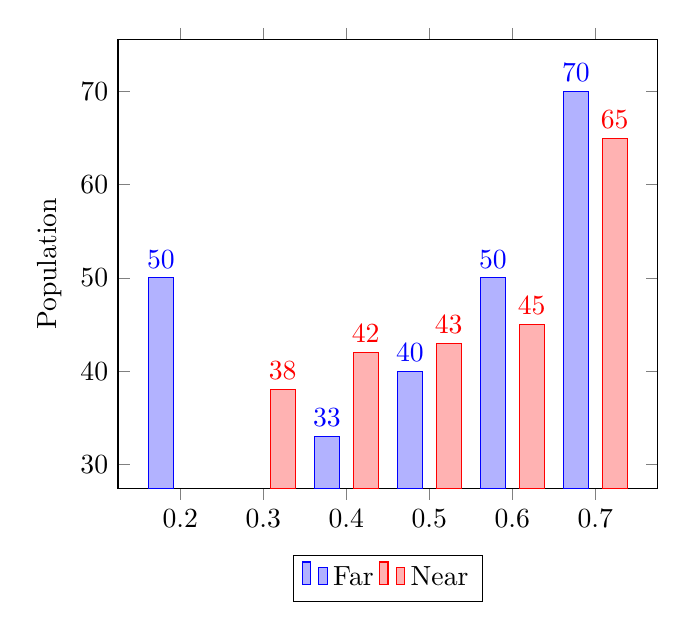
\begin{tikzpicture}
  \begin{axis}
    [
    x tick label style={
      /pgf/number format/1000 sep=},
    ylabel=Population,
    enlargelimits=0.15,
    legend style={at={(0.5,-0.15)},
      anchor=north,legend columns=-1},
    ybar=5pt,% configures ‘bar shift’
    bar width=9pt,
    nodes near coords,
    point meta=y % the displayed number
    ]
    \addplot
    coordinates {(0.2,50) (0.4,33)
      (0.5,40) (0.6,50) (0.7,70)};
    \addplot
    coordinates {(0.3,38) (0.4,42)
      (0.5,43) (0.6,45) (0.7,65)};
    \legend{Far,Near}
  \end{axis}
    \label{experiment:fig:threshold}
  \end{tikzpicture}
  
  从\reffig{experiment:fig:threshold}所示的实验结果中,我们可以看到聚类时设置的阈
  值大小不仅会影响聚类的个数,对后续的模板生成也有较大的影响。通过分析,我们可以
  得到以下几个结论:%TODO: 分析!
\begin{itemize}
\item 聚类时的阈值越小,
\end{itemize}

\section{内容抽取模块实验}
为了将我们的系统部署到实际的生产环境中,我们在测试集上进行了实验。首先是人工对每
个模板进行标注,然后利用标注好的模板,对每个新的网页(测试集)进行内容抽取,我们
将抽取的内容使用XML格式保存下来。\reffig{experiment:fig:xmloutput}是我们保存到
XML中的结果的截图。
\begin{figure}[hb]
  \centering
  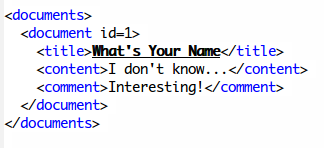
\includegraphics[width=0.5\textwidth]{experiment06/xmloutput}
  \caption{XML保存的结果截图}
  \label{experiment:fig:xmloutput}
\end{figure}

从\reffig{experiment:fig:xmloutput}可以看到,我们。%TODO:
\section{实验结果总结}
\label{sec:analysis}
对以上的实验结果,我们做以下的总结:%TODO
\begin{itemize}
\item 在预处理模块
\end{itemize}

%%% Local Variables: 
%%% mode: latex
%%% TeX-master: "../main"
%%% End: 
